\documentclass[11pt,a4paper]{article}
\usepackage[utf8]{inputenc}
\usepackage[T1]{fontenc}
\usepackage{newtxtext,newtxmath}
\usepackage[spanish,es-nodecimaldot,es-noshorthands,es-tabla]{babel}
\usepackage[a4paper,left=2.2cm,right=2.2cm,top=2.1cm,bottom=2.1cm,headheight=14pt,includehead,includefoot]{geometry}
\usepackage{microtype}
\usepackage{setspace}\setstretch{1.13}
\usepackage[parfill]{parskip}
\usepackage{amsmath}
\usepackage{graphicx}
\usepackage{booktabs}
\usepackage{tabularx}
\usepackage{array}
\usepackage{xcolor}
\usepackage{tikz}
\usetikzlibrary{arrows.meta,positioning,calc}
\usepackage[ruled,vlined,linesnumbered]{algorithm2e}
\usepackage{float}
\usepackage{caption}
\renewcommand{\topfraction}{0.88}
\renewcommand{\bottomfraction}{0.85}
\renewcommand{\textfraction}{0.10}
\renewcommand{\floatpagefraction}{0.82}
\widowpenalty=10000
\clubpenalty=10000
\displaywidowpenalty=10000
\setlength{\intextsep}{10pt plus 2pt minus 2pt}
\setlength{\textfloatsep}{12pt plus 2pt minus 2pt}
\setlength{\abovecaptionskip}{6pt}
\setlength{\belowcaptionskip}{4pt}
\captionsetup{font=small,labelfont=bf,margin=0.5cm}
\usepackage{titlesec}
\titleformat{\section}{\Large\bfseries}{\thesection.}{0.6em}{}
\titleformat{\subsection}{\large\bfseries}{\thesubsection.}{0.6em}{}
\titlespacing*{\section}{0pt}{1.6ex plus .5ex}{0.9ex}
\titlespacing*{\subsection}{0pt}{1.3ex plus .4ex}{0.5ex}
\usepackage{fancyhdr}
\pagestyle{fancy}\fancyhf{}
\fancyhead[L]{\small\itshape Proyecto 5: KNN paralelo con MPI}
\fancyhead[R]{\small\itshape CS4052 -- Computación Paralela y Distribuida}
\fancyfoot[C]{\small\thepage}
\renewcommand{\headrulewidth}{0.4pt}
\definecolor{utecazul}{HTML}{1F3A5F}
\definecolor{cajafondo}{HTML}{F2F5F9}
\usepackage[hidelinks]{hyperref}
\usepackage{url}
\SetAlgorithmName{Algoritmo}{algoritmo}{Lista de algoritmos}
\SetKwInput{KwIn}{Entrada}\SetKwInput{KwOut}{Salida}
\SetKwFor{ForAllPar}{forall}{pardo}{end}
\SetKwComment{tcp}{$\triangleright$\ }{}
\SetAlFnt{\small}\SetAlCapFnt{\small}\SetAlCapNameFnt{\small}
\graphicspath{{figs/}}
\newcommand{\ntr}{n_{tr}}
\newcommand{\nte}{n_{te}}
\newcommand{\tsub}[1]{T_{\mathrm{#1}}}
\renewcommand{\arraystretch}{1.08}
\setlength{\tabcolsep}{6pt}

\begin{document}
\begin{titlepage}
\centering
\vspace*{0.6cm}
{\Large\bfseries Universidad de Ingeniería y Tecnología (UTEC)\par}
\vspace{0.15cm}
{\large Facultad de Ciencia de la Computación\par}
\vspace{0.5cm}
{\large CS4052 -- Computación Paralela y Distribuida -- 2026-II\par}
\vspace{0.6cm}
{\color{utecazul}\rule{\linewidth}{1.2pt}\par}
\vspace{1.4cm}
{\Large Informe final de proyecto\par}
\vspace{0.6cm}
{\LARGE\bfseries\color{utecazul} Proyecto 5: paralelización del clasificador KNN\\[2pt] sobre \texttt{load\_digits} mediante MPI (\texttt{mpi4py})\par}
\vspace{1.4cm}
{\color{utecazul}\rule{\linewidth}{1.2pt}\par}
\vspace{1.6cm}
{\large\bfseries Integrantes y participación\par}
\vspace{0.3cm}
{\large
\begin{tabular}{l@{\hspace{1.5cm}}r}
Juan David Velo Poma & 100\,\%\\
Farid Jack Aquino Castro & 100\,\%\\
Josue Nehemias Velo Poma & 100\,\%\\
\end{tabular}\par}
\vfill
\begin{tabular}{@{}r@{\hspace{0.4cm}}l@{}}
\textbf{Profesor:} & José Fiestas, PhD\\
\textbf{Fecha:} & 22 de noviembre de 2026\\
\textbf{Entorno de cómputo:} & Clúster Khipu (UTEC), un nodo con 16 núcleos físicos\\
\textbf{Código:} & \url{https://github.com/Juan-Velo/cpd_proyecto_final}\\
\end{tabular}
\vspace{0.8cm}
\end{titlepage}

\pagenumbering{roman}
\tableofcontents
\thispagestyle{fancy}
\clearpage
\pagenumbering{arabic}

\noindent\colorbox{cajafondo}{\begin{minipage}{\dimexpr\linewidth-2\fboxsep\relax}
\vspace{0.3em}
{\large\bfseries\color{utecazul} Resumen}\par\vspace{0.4em}
Paralelizamos con MPI el clasificador KNN de \texttt{knn\_digits\_sec.py} siguiendo el DAG del enunciado: Scatter de los datos de entrenamiento, Bcast de los datos de prueba, cálculo local de los $k$ vecinos y Gather de los candidatos. Resultados medidos en Khipu:
\begin{itemize}\setlength{\itemsep}{1pt}
\item \textbf{Correcto:} las tres versiones beta dan exactamente las mismas 360 predicciones que el código original (exactitud 0.9833) para todo $p$.
\item \textbf{Rendimiento:} con el conjunto grande ($\ntr=91\,968$) y 16 procesos, speedup $S=6.61$, eficiencia $E=0.41$ y 58.3\,GFLOP/s. La comunicación es como máximo el 1.1\,\% del tiempo.
\item \textbf{Cantidad óptima de procesos:} la teoría da $p^*\approx8$ para \texttt{load\_digits}, lo que coincide con lo medido. Para los conjuntos grandes, $p^*$ es mayor que 16, así que conviene usar los 16 núcleos.
\item \textbf{Límite:} la pérdida de eficiencia no viene de MPI sino del cómputo: con 16 procesos en un mismo nodo, cada proceso calcula unas 2.5 veces más lento. La causa más probable es que todos comparten la memoria del nodo (U1.1, U4.5), aunque no lo medimos directamente.
\end{itemize}
\vspace{0.1em}
\end{minipage}}
\vspace{0.6em}

% =====================================================================
\section{Introducción}
\textbf{El problema.} KNN clasifica un punto $q$ con la etiqueta más frecuente entre sus $k$ vecinos más cercanos \cite{fix1951,cover1967}. No construye ningún modelo: todo el costo está en calcular las distancias entre cada punto de prueba y todos los puntos de entrenamiento. El conjunto \texttt{load\_digits} \cite{sklearn} tiene 1797 imágenes de $8\times8$ píxeles ($d=64$ valores enteros entre 0 y 16, 10 clases). Con \texttt{test\_size=0.2} quedan $\ntr=1437$ puntos de entrenamiento y $\nte=360$ de prueba; usamos $k=3$.

\textbf{Código de partida.} \texttt{knn\_digits\_sec.py} calcula cada distancia en un bucle de Python, ordena con \texttt{argsort} y vota con \texttt{Counter}. Su exactitud es 0.9833 y en Khipu tarda 1.988\,s.

\textbf{Solución planteada.} Seguimos el DAG del enunciado (Fig.~\ref{fig:dag}): el proceso 0 reparte los datos de entrenamiento entre los $p$ procesos (Scatter) y envía todos los datos de prueba a todos (Bcast). Cada proceso calcula sus distancias y se queda con sus $k$ mejores candidatos por consulta. Al final el proceso 0 junta los candidatos (Gather) y vota.

\textbf{Cambio respecto a la entrega parcial.} En la entrega parcial habíamos propuesto la distribución inversa: Bcast de $X_{tr}$ y Scatter de $X_{te}$, con otra notación ($s$ procesos, $n$ y $m$ puntos). En esta entrega seguimos el DAG del enunciado porque comunica mucho menos cuando $\ntr\gg\nte$ (lo medimos en la Sec.~\ref{sec:variantes}: 4.7 veces menos comunicación). Por eso las fórmulas de comunicación de este informe son distintas a las de la entrega parcial: ahora el Bcast envía $X_{te}$, no $X_{tr}$. La Tabla~\ref{tab:notacion} fija la notación actual.

\begin{table}[htbp]
\centering\small
\caption{Notación.}\label{tab:notacion}
\begin{tabular}{@{}ll@{}}\toprule
Símbolo & Significado\\\midrule
$\ntr$, $\nte$ & número de puntos de entrenamiento y de prueba\\
$d$, $k$ & dimensión ($d=64$) y número de vecinos ($k=3$)\\
$p$, $r$ & número de procesos MPI y rango de un proceso ($0,\dots,p-1$)\\
$\alpha$, $\beta$ & latencia por mensaje y tiempo por byte (U6.1)\\
$W$, $T_\infty$ & trabajo y span (U1.3)\\
$T_p$ & tiempo paralelo con $p$ procesos ($T_1$: con un proceso)\\
$\tsub{comp}$, $\tsub{comm}$ & tiempo de cómputo y de comunicación\\
$S$, $E$ & speedup $T_1/T_p$ y eficiencia $S/p$ (U2.1)\\\bottomrule
\end{tabular}
\end{table}

\begin{figure}[htbp]
\centering
\begin{tikzpicture}[
  node distance=10mm and 5mm, >={Stealth[length=2.2mm]},
  task/.style={draw, rounded corners=2pt, fill=gray!8, align=center, font=\small, minimum height=8mm, inner sep=3pt},
  cost/.style={font=\small, inner sep=1pt}]
\node[task, minimum width=38mm] (init) {Datos iniciales\\ $X_{tr},y_{tr},X_{te}$ en $P_0$};
\node[task, below left=12mm and 2mm of init] (d0) {distancias, top-$k$\\ $P_0$};
\node[task, right=5mm of d0] (d1) {distancias, top-$k$\\ $P_1$};
\node[font=\large, right=3mm of d1] (dots) {$\cdots$};
\node[task, right=3mm of dots] (dp) {distancias, top-$k$\\ $P_{p-1}$};
\node[task, below=12mm of d1.south east, anchor=north, xshift=6mm, minimum width=38mm] (vote) {Voto por mayoría en $P_0$\\ ($k$ mejores de $p\,k$ candidatos)};
\foreach \n in {d0,d1,dp} {\draw[->] (init) -- (\n); \draw[->] (\n) -- (vote);}
\node[cost, color=blue!60!black, anchor=east] at ($(init.west)+(-2mm,-2mm)$) {Scatter de $X_{tr}$};
\node[cost, color=blue!60!black, anchor=west] at ($(init.east)+(2mm,-2mm)$) {Bcast de $X_{te}$};
\node[cost, color=red!60!black, anchor=east] at ($(d0.west)+(-4mm,0)$) {Cómputo: $O\!\left(\tfrac{\ntr\nte d}{p}\right)$};
\node[cost, color=blue!60!black, anchor=west] at ($(vote.east)+(2mm,1.5mm)$) {Gather};
\end{tikzpicture}
\caption{DAG del enunciado. Azul: comunicación; rojo: cómputo. Es un DAG secuencial-paralelo (SPA, U1.3): reparto de datos, $p$ tareas independientes y recolección.}
\label{fig:dag}
\end{figure}

% =====================================================================
\section{Método}
\subsection{Diseño}
Usamos la metodología de Foster (U1.2):
\begin{itemize}
\item \emph{Particionamiento:} cada distancia (consulta $j$, punto $i$) es una tarea independiente.
\item \emph{Comunicación:} solo al inicio (Scatter y Bcast) y al final (Gather).
\item \emph{Aglomeración:} cada proceso toma un bloque contiguo de puntos de entrenamiento y lo compara con todas las consultas. Así envía solo $k$ candidatos por consulta, no todas sus distancias.
\item \emph{Mapeo:} un bloque por proceso. Si $\ntr$ no es divisible entre $p$, los primeros $\ntr\bmod p$ procesos reciben un punto más.
\end{itemize}
Según Flynn es MIMD, programado como SPMD (el mismo programa en todos los procesos). Es un particionamiento de datos con tareas separables (U2.4).

\subsection{Pseudocódigos: secuencial, PRAM y MPI}\label{sec:pseudo}
El Alg.~\ref{alg:seq} resume el código secuencial de partida.

\begin{algorithm}[htbp]
\caption{KNN secuencial (\texttt{knn\_digits\_sec.py})}\label{alg:seq}
\KwIn{$X_{tr},y_{tr},X_{te},y_{te}$ (\texttt{train\_test\_split} con \texttt{test\_size}=0.2), $k=3$}
\KwOut{exactitud y tiempo}
$t_{\mathrm{ini}}\leftarrow\texttt{time()}$\;
\For{$j\leftarrow1$ \KwTo $\nte$}{
  \For{$i\leftarrow1$ \KwTo $\ntr$}{$D[i]\leftarrow\sqrt{\sum_{l=1}^{d}(X_{te}[j,l]-X_{tr}[i,l])^2}$ \tcp*{$3d$ FLOP}}
  $K\leftarrow\texttt{argsort}(D)[1..k]$\;
  $\hat y[j]\leftarrow$ etiqueta más frecuente en $y_{tr}[K]$ \tcp*{\texttt{Counter}}
}
exactitud $\leftarrow\frac1{\nte}\sum_j[\hat y[j]=y_{te}[j]]$;\quad $t_{\mathrm{fin}}\leftarrow\texttt{time()}$\;
\Return{exactitud, $t_{\mathrm{fin}}-t_{\mathrm{ini}}$}
\end{algorithm}

\textbf{PRAM} (Alg.~\ref{alg:pram}). Todas las distancias son independientes, así que el modelo ideal usa un procesador por par (consulta, punto). Es una PRAM CREW (U2.2): todos leen $X_{tr}$ y $X_{te}$ a la vez (lectura concurrente), pero cada procesador escribe solo en su propia celda (escritura exclusiva).

\begin{algorithm}[htbp]
\caption{KNN en PRAM CREW ($\nte\cdot\ntr$ procesadores)}\label{alg:pram}
\KwIn{$X_{tr},\,y_{tr},\,X_{te}$, $k$}
\KwOut{predicciones $\hat y$}
\ForAllPar{$(j,i)\in\{1,\dots,\nte\}\times\{1,\dots,\ntr\}$}{
  $D[j,i]\leftarrow\sqrt{\sum_{l=1}^{d}(X_{te}[j,l]-X_{tr}[i,l])^2}$ \tcp*{suma en árbol: $O(\log d)$}
}
\ForAllPar{$j\in\{1,\dots,\nte\}$}{
  $N_j\leftarrow$ los $k$ menores de $D[j,\cdot]$ \tcp*{$k$ reducciones de mínimo: $O(k\log\ntr)$}
  $\hat y[j]\leftarrow$ etiqueta más frecuente en $y_{tr}[N_j]$\;
}
\end{algorithm}

\textbf{Versión MPI} (Alg.~\ref{alg:mpi}). Es la que implementamos (beta2 y beta3) y sigue el DAG de la Fig.~\ref{fig:dag}.

\begin{algorithm}[htbp]
\caption{KNN con MPI según el DAG ($p$ procesos, rango $r$)}\label{alg:mpi}
\KwIn{$X_{tr},y_{tr},X_{te}$ en $P_0$; $k$}
\KwOut{$\hat y$ y exactitud en $P_0$}
$n_r\leftarrow\lfloor\ntr/p\rfloor+[\,r<\ntr\bmod p\,]$ \tcp*{tamaño del bloque de $P_r$}
$(X_{tr}^{(r)},y_{tr}^{(r)})\leftarrow\textsc{Scatter}(X_{tr},y_{tr})$ \tcp*{\texttt{comm.scatter}}
$X_{te}\leftarrow\textsc{Bcast}(X_{te})$ \tcp*{\texttt{comm.bcast}}
\ForAllPar{$r\leftarrow0$ \KwTo $p-1$}{
  \For{$j\leftarrow1$ \KwTo $\nte$}{
    \For{$i\leftarrow1$ \KwTo $n_r$}{$D_r[j,i]\leftarrow\|X_{te}[j]-X^{(r)}_{tr}[i]\|_2$ \tcp*{$3d$ FLOP}}
    $K_r[j]\leftarrow$ los $k$ menores: (distancia, índice global, etiqueta)\;
  }
}
$(K_0,\dots,K_{p-1})\leftarrow\textsc{Gather}(K_r)$ \tcp*{\texttt{comm.gather}: $3k\nte$ valores por proceso}
\If{$r=0$}{
  \For{$j\leftarrow1$ \KwTo $\nte$}{
    $N_j\leftarrow$ los $k$ menores entre los $p\,k$ candidatos;\quad $\hat y[j]\leftarrow$ etiqueta más frecuente\;
  }
  exactitud $\leftarrow\frac1{\nte}\sum_j[\hat y[j]=y_{te}[j]]$\;
}
\end{algorithm}

\textbf{¿Por qué el resultado es igual al secuencial?} Cada uno de los $k$ vecinos globales está en algún bloque, y dentro de ese bloque también es de los $k$ más cercanos. Por eso aparece entre los $p\,k$ candidatos que recibe $P_0$, y la elección final es la misma que la del secuencial. Ordenamos por (distancia, índice), así que los empates se resuelven igual para cualquier $p$.

\subsection{Complejidad teórica}\label{sec:complejidad}
\textbf{Cómputo.} Cada distancia cuesta $3d$ FLOP ($d$ restas, $d$ cuadrados y $d$ sumas, contando la raíz como una operación). Según U1.3 y U2.2:
\begin{align}
W&=3d\,\ntr\nte=O(\ntr\nte d), \qquad T_\infty=O(\log d+k\log\ntr),\label{eq:work}\\
T_p^{\mathrm{PRAM}}&\le\frac{W}{p}+T_\infty\qquad\text{(teorema de Brent).}\label{eq:brent}
\end{align}
En la versión MPI se agrega la fusión en $P_0$: cada consulta elige entre $p\,k$ candidatos. Ese paso no se reparte, así que crece con $p$:
\begin{equation}
\tsub{comp}=O\!\left(\frac{\ntr\nte d}{p}\right)+O(\nte\,k\,p).\label{eq:tcomp}
\end{equation}

\textbf{Comunicación.} Usamos las fórmulas de U6.1: Bcast en árbol binomial, $\log_2p\,(\alpha+m\beta)$, y Scatter/Gather, $p(\alpha+\frac mp\beta)+(p-1)(\alpha+\frac mp\beta)=(2p-1)(\alpha+\frac mp\beta)$. El tamaño $m$ va en bytes (8 por valor):
\begin{align}
\tsub{Scatter}&=2(2p-1)\alpha+\tfrac{2p-1}{p}\,8\ntr(d+1)\beta &&\text{($X_{tr}$ y $y_{tr}$)},\nonumber\\
\tsub{Bcast}&=\log_2p\,(\alpha+8\nte d\beta) &&\text{($X_{te}$)},\label{eq:comm}\\
\tsub{Gather}&=(2p-1)(\alpha+24k\nte\beta) &&\text{($3k\nte$ valores por proceso)}.\nonumber
\end{align}

\textbf{Tiempo paralelo.} Si sumamos (\ref{eq:tcomp}) y (\ref{eq:comm}) y agrupamos los términos según cómo dependen de $p$, queda:
\begin{equation}
T_p\approx\frac{A}{p}+B\,p+C\log_2p+D,\label{eq:tp}
\end{equation}
\begin{itemize}\setlength{\itemsep}{1pt}
\item $A=c_1\ntr\nte d$: las distancias, que se reparten entre los $p$ procesos;
\item $B=c_2\nte k+6\alpha+48k\nte\beta$: lo que \emph{crece} con $p$, es decir, la fusión en $P_0$, el Gather y los arranques de mensajes;
\item $C=\alpha+8\nte d\beta$: el Bcast de $X_{te}$;
\item $D\approx16\ntr(d+1)\beta$: los bytes del Scatter, que casi no dependen de $p$.
\end{itemize}

\textbf{Métricas} (U2.1, U6.2): $S=T_1/T_p$, $E=S/p$ y $\text{GFLOP/s}=W/(T_p\cdot10^9)$, con $W=3d\,\ntr\nte$. Esta es la región paralelizable que pide el enunciado y se basa en la fórmula de la distancia euclidiana.

\subsection{Normalización de la expresión teórica}\label{sec:norm}
La Ec.~(\ref{eq:tp}) da la \emph{forma} del tiempo, pero no los segundos. Para convertirla en segundos hay que hallar las constantes a partir de las mediciones:
\begin{enumerate}
\item $c_1$ = tiempo por cada término $\ntr\nte d$. Lo obtenemos de la corrida con \textbf{un solo proceso} ($p=1$) de los tres tamaños: $c_1=3.05\times10^{-10}$\,s. Equivale a $3/c_1=9.8$\,GFLOP/s por núcleo, dentro del rango de 4--12\,GFLOP/s por núcleo que da U2.1.
\item $c_2$ = tiempo por candidato en la fusión. Sale del tiempo medido del voto en $P_0$: $c_2=9.0\times10^{-8}$\,s.
\item $\alpha$ y $\beta$: por mínimos cuadrados sobre el tiempo de comunicación medido. Dan $\alpha=6.5\,\mu$s y $\beta=1.3\times10^{-10}$\,s/byte (7.7\,GB/s).
\end{enumerate}
Con $c_1$ tomado de $p=1$, la curva teórica es el caso \emph{ideal}: el cómputo baja exactamente como $1/p$. Si lo medido se separa de esa curva, sabemos que algo escala peor que la teoría.

\emph{Ejemplo} (conjunto grande, $\ntr=91\,968$, $\nte=3600$, $p=16$): $A=c_1\ntr\nte d=6.472$\,s, $B=1.08\times10^{-3}$\,s, $C=2.5\times10^{-4}$\,s y $D=0.0125$\,s. Entonces
\[
T_{16}\approx\tfrac{6.472}{16}+1.08\times10^{-3}\cdot16+2.5\times10^{-4}\cdot4+0.0125=0.404+0.017+0.001+0.012=0.435\ \text{s}.
\]
Lo medido es 1.091\,s. Explicamos la diferencia en la Sec.~\ref{sec:tiempos}.

\subsection{Cantidad óptima de procesos}\label{sec:pstar}
En la Ec.~(\ref{eq:tp}), el término $A/p$ baja al aumentar $p$ y el término $B\,p$ sube. El óptimo $p^*$ es el punto donde la derivada vale cero. Es el mismo procedimiento con el que U6.1 calcula el número óptimo de trozos $k$ del broadcast \emph{pipelined}:
\[
\frac{dT_p}{dp}=-\frac{A}{p^2}+B+\frac{C}{p\ln2}=0.
\]
El término $C$ es muy pequeño frente a $A$ y $B$; si lo despreciamos:
\begin{equation}
p^*\approx\sqrt{\frac{A}{B}}.\label{eq:pstar}
\end{equation}
Si se mantiene $C$, $p^*$ cambia menos de un 2\,\%. Los valores para cada tamaño están en la Sec.~\ref{sec:resp}.

\subsection{Versiones beta y validación}\label{sec:betas}
El código se desarrolló en tres pasos (Tabla~\ref{tab:betas}). Todas las mediciones de la Sec.~\ref{sec:res} usan \textbf{beta3}, la versión final.

\begin{table}[htbp]
\centering\small
\caption{Versiones beta. Cada una se validó contra la anterior.}\label{tab:betas}
\begin{tabularx}{\linewidth}{@{}>{\raggedright\arraybackslash}p{3.55cm}>{\raggedright\arraybackslash}X>{\raggedright\arraybackslash}p{3.3cm}@{}}\toprule
Archivo & Qué hace & Validación\\\midrule
\texttt{beta1\_secuencial.py} & Código original y una versión vectorizada con NumPy. Vectorizar baja el tiempo de \texttt{load\_digits} de 1.988\,s a 12.7\,ms. & 360/360 predicciones iguales al original.\\\addlinespace
\texttt{beta2\_mpi\_basico.py} & Primera versión MPI del DAG (Alg.~\ref{alg:mpi}) con \texttt{comm.scatter}, \texttt{comm.bcast} y \texttt{comm.gather}, como pide el enunciado. Mantiene el bucle original de distancias. & Igual a beta1 con $p=1$ a 16.\\\addlinespace
\texttt{beta3\_mpi\_}\linebreak\texttt{optimizado.py} & Versión final: las mismas colectivas, pero sobre arreglos NumPy (\texttt{Scatterv}, \texttt{Bcast}, \texttt{Gather}); distancias calculadas como producto de matrices (U6.3) y selección con \texttt{argpartition}. Mide por separado cómputo y comunicación con \texttt{MPI.Wtime}. & Igual a beta1 con $p=1$ a 16.\\\bottomrule
\end{tabularx}
\end{table}

\textbf{Validación} (\texttt{tests/validate\_knn.py}, job 64269 en Khipu): \textbf{129/129} comprobaciones correctas. Las versiones MPI reproducen las 360 predicciones originales con $p\in\{1,2,3,4,5,7,8,16\}$, incluido un caso con $\ntr$ no divisible entre $p$. Además, la partición en bloques se comprobó para $p=1,\dots,17$, 32 y 64.

\textbf{Producto de matrices exacto.} beta3 usa $\|q-x\|^2=\|q\|^2+\|x\|^2-2\,q\cdot x$. Como los píxeles son enteros entre 0 y 16, todos esos valores son enteros pequeños ($\le64\cdot16^2$), y en \texttt{float64} no hay redondeo. Por eso las distancias son idénticas a las del bucle original.

\subsection{Aumento del tamaño del problema}\label{sec:aug}
El enunciado pide aumentar $n$. Para eso generamos copias de \texttt{load\_digits} con un poco de ruido (gaussiano con $\sigma=1$, redondeado a enteros entre 0 y 16, con semilla fija), por separado para el entrenamiento y para la prueba. Los tamaños usados son:
\begin{itemize}\setlength{\itemsep}{1pt}
\item \textbf{load\_digits:} original, $\ntr=1437$, $\nte=360$;
\item \textbf{Mediano:} $\ntr=22\,992$ ($16\times$), $\nte=3600$ ($10\times$);
\item \textbf{Grande:} $\ntr=91\,968$ ($64\times$), $\nte=3600$;
\item \textbf{Serie con tamaño variable:} $\ntr=11\,496\cdot p$, para que cada proceso tenga siempre el mismo trabajo (Sec.~\ref{sec:escala}).
\end{itemize}
La exactitud se mantiene entre 0.980 y 0.983 en todos los tamaños (Sec.~\ref{sec:acc}).

% =====================================================================
\section{Resultados y análisis}\label{sec:res}
\textbf{Entorno.} Clúster Khipu, un nodo con 2 procesadores Intel Xeon Gold 6130 (16 núcleos cada uno). La cuenta de pregrado permite 16 núcleos físicos, así que $p\le16$. Software: Python 3.11, NumPy, mpi4py y MPICH. Cada proceso usa un solo núcleo. Cada punto es el promedio de 5 repeticiones.

\subsection{Tiempos de ejecución, cómputo y comunicación}\label{sec:tiempos}
\begin{figure}[htbp]
\centering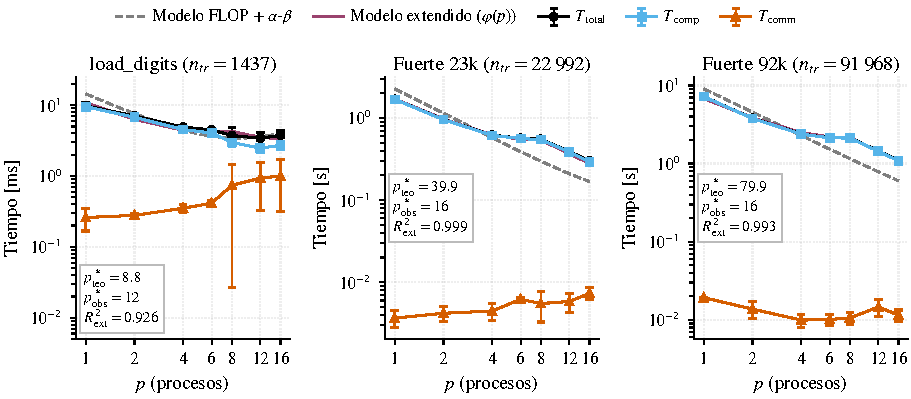
\includegraphics[width=\textwidth]{tiempos_vs_p}
\caption{Tiempo total, de cómputo y de comunicación frente a $p$ para los tres tamaños. Líneas continuas: medido. Líneas discontinuas: modelo teórico normalizado (Ec.~\ref{eq:tp}).}
\label{fig:tiempos}
\end{figure}

La Fig.~\ref{fig:tiempos} compara lo medido con la teoría:
\begin{enumerate}
\item \textbf{La comunicación es pequeña y sigue la teoría.} En los conjuntos Mediano y Grande es como máximo el 2.5\,\% y el 1.1\,\% del tiempo total, y su valor medido está cerca de la curva teórica de U6.1. En \texttt{load\_digits} el cómputo es tan pequeño (unos 10\,ms) que la comunicación llega al 27\,\% del total con $p=16$.
\item \textbf{Con $p=1$ la teoría acierta.} El error es menor al 11\,\% en los tres tamaños.
\item \textbf{Al aumentar $p$, el cómputo baja más lento que $1/p$.} En los conjuntos Mediano y Grande, el tiempo medido dividido entre el teórico pasa de 1.0--1.1 con $p=1$ a $\approx$2.5 desde $p=8$. La diferencia está en el cómputo, no en la comunicación.
\end{enumerate}

\textbf{¿Por qué el cómputo no baja como $1/p$?} Lo comprobamos con la serie de tamaño variable (Sec.~\ref{sec:escala}). Ahí cada proceso tiene \emph{siempre el mismo trabajo}, y aun así su tiempo de cómputo sube de 0.84\,s ($p=1$) a 2.11\,s ($p=16$): 2.5 veces, el mismo factor que vemos arriba. Como el trabajo no cambió, la causa no es el algoritmo ni MPI, sino que los 16 procesos comparten los recursos del nodo. U1.1 señala que el acceso a memoria es el cuello de botella frente al cómputo (\emph{memory wall}). U4.5 advierte que más procesos o hilos no significan más rendimiento, porque comparten el ancho de banda de memoria. No medimos contadores de hardware, así que no podemos separar las causas exactas.

\subsection{Speedup y eficiencia}\label{sec:speedup}
\begin{figure}[htbp]
\centering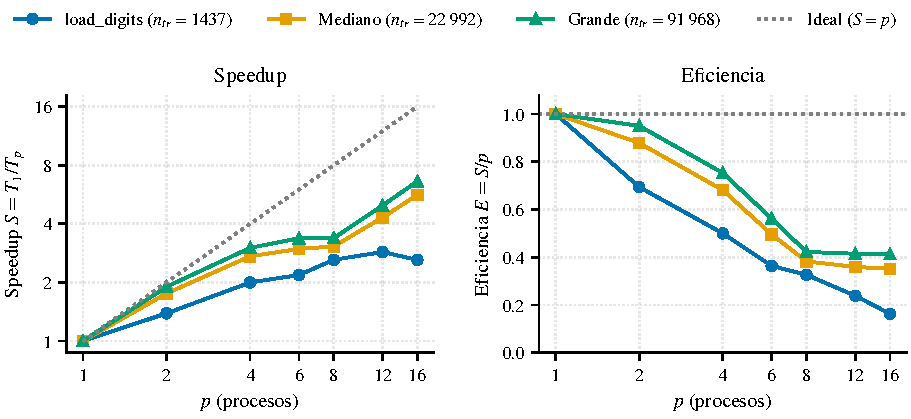
\includegraphics[width=\textwidth]{speedup_eficiencia}
\caption{Speedup y eficiencia con tamaño fijo y $p$ creciente (escalabilidad fuerte). La línea punteada es el caso ideal $S=p$, $E=1$.}
\label{fig:speedup}
\end{figure}

\begin{table}[htbp]
\centering\small
\caption{Tiempo, speedup y eficiencia ($S=T_1/T_p$, $E=S/p$). $T_1$ es beta3 con un proceso.}\label{tab:strong}
\setlength{\tabcolsep}{4pt}
\begin{tabular}{@{}r|rrr|rrr|rrr@{}}\toprule
& \multicolumn{3}{c|}{load\_digits} & \multicolumn{3}{c|}{Mediano ($\ntr=22\,992$)} & \multicolumn{3}{c}{Grande ($\ntr=91\,968$)}\\
$p$ & $T_p$ [ms] & $S$ & $E$ & $T_p$ [s] & $S$ & $E$ & $T_p$ [s] & $S$ & $E$\\\midrule
1 & 9.75 & 1.00 & 1.00 & 1.684 & 1.00 & 1.00 & 7.208 & 1.00 & 1.00\\
2 & 7.02 & 1.39 & 0.69 & 0.958 & 1.76 & 0.88 & 3.793 & 1.90 & 0.95\\
4 & 4.88 & 2.00 & 0.50 & 0.618 & 2.72 & 0.68 & 2.394 & 3.01 & 0.75\\
6 & 4.47 & 2.18 & 0.36 & 0.566 & 2.97 & 0.50 & 2.139 & 3.37 & 0.56\\
8 & 3.73 & 2.61 & 0.33 & 0.550 & 3.06 & 0.38 & 2.134 & 3.38 & 0.42\\
12 & 3.40 & 2.87 & 0.24 & 0.390 & 4.31 & 0.36 & 1.449 & 4.98 & 0.41\\
16 & 3.74 & 2.61 & 0.16 & 0.299 & 5.63 & 0.35 & 1.091 & 6.61 & 0.41\\\bottomrule
\end{tabular}
\end{table}

La Fig.~\ref{fig:speedup} y la Tabla~\ref{tab:strong} muestran que:
\begin{itemize}
\item cuanto más grande es el problema, mejor escala: con $p=16$, $S=2.61$ en \texttt{load\_digits}, 5.63 en Mediano y 6.61 en Grande;
\item la eficiencia cae hasta $p=8$ y luego se mantiene en 0.35--0.41 en los conjuntos grandes. Esa caída es la del cómputo explicada en la Sec.~\ref{sec:tiempos};
\item en \texttt{load\_digits} el speedup deja de crecer después de $p\approx8$--12, porque hay muy poco trabajo para repartir.
\end{itemize}

\subsection{FLOP/s frente a $p$}\label{sec:flops}
Como en U6.2, contamos los FLOP con la fórmula del algoritmo ($W=3d\,\ntr\nte$) y los dividimos entre el tiempo medido. Así lo pide el enunciado: FLOP basados en la fórmula de la distancia euclidiana. Para el conjunto Grande, $W=6.36\times10^{10}$ FLOP. Son GFLOP/s \emph{equivalentes}: beta3 obtiene la misma distancia con un producto de matrices, que ejecuta unas $2d$ operaciones por par en lugar de $3d$. Por eso no son operaciones contadas por el hardware.

\begin{figure}[htbp]
\centering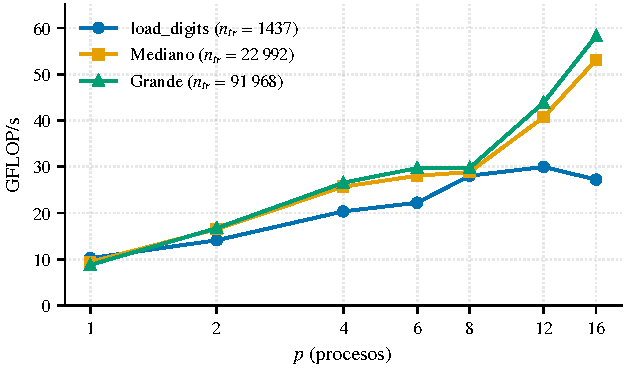
\includegraphics[width=0.7\textwidth]{gflops_vs_p}
\caption{GFLOP/s $=3d\,\ntr\nte/(T_p\cdot10^9)$ frente a $p$.}
\label{fig:flops}
\end{figure}

En la Fig.~\ref{fig:flops}, el conjunto Grande pasa de 8.8\,GFLOP/s con $p=1$ a \textbf{58.3\,GFLOP/s} con $p=16$, y el Mediano de 9.4 a 53.1. En \texttt{load\_digits} se llega como máximo a 30\,GFLOP/s ($p=12$) y luego baja, por el mismo motivo que el speedup.

\subsection{Respuesta: cantidad óptima de procesos}\label{sec:resp}
La Tabla~\ref{tab:pstar} aplica la Ec.~(\ref{eq:pstar}) a cada tamaño.

\begin{table}[htbp]
\centering\small
\caption{Cantidad óptima de procesos: teoría ($p^*=\sqrt{A/B}$) frente a medición.}\label{tab:pstar}
\begin{tabular}{@{}lrrrl@{}}\toprule
Tamaño & $A$ [s] & $B$ [s] & $p^*\approx\sqrt{A/B}$ & Medido\\\midrule
load\_digits & $1.01\times10^{-2}$ & $1.43\times10^{-4}$ & 8.4 & mínimo en $p=12$; $p=8$ y 16 dentro de $1\sigma$\\
Mediano & 1.62 & $1.08\times10^{-3}$ & 38.7 & sigue bajando hasta $p=16$\\
Grande & 6.47 & $1.08\times10^{-3}$ & 77.4 & sigue bajando hasta $p=16$\\\bottomrule
\end{tabular}
\end{table}

\begin{itemize}
\item \textbf{load\_digits:} la teoría da $p^*\approx8$. El mínimo medido está en $p=12$ ($3.40\pm0.65$\,ms), pero $T_8=3.73\pm1.11$ y $T_{16}=3.74\pm0.69$\,ms: las diferencias son menores que la variación entre repeticiones, así que a partir de $p=8$ el tiempo ya no mejora de forma apreciable. \textbf{Estimación: 8 procesos}, porque da el mismo tiempo con menos recursos.
\item \textbf{Mediano y Grande:} $p^*$ (39 y 77) es mayor que los 16 núcleos disponibles, y el tiempo sigue bajando hasta $p=16$. \textbf{Estimación: usar todos los núcleos físicos (16).} Como $A$ crece con $\ntr$, un problema más grande admite más procesos.
\item \textbf{Hyper-threading:} con 2 procesos por núcleo ($p=32$ en 16 núcleos), el conjunto Grande tarda 1.208\,s, más que los 1.091\,s con $p=16$. U4.5 lo anticipa: un hilo extra de hardware (SMT) no equivale a un núcleo real.
\end{itemize}

\subsection{Escalabilidad con tamaño variable del problema}\label{sec:escala}
\begin{figure}[htbp]
\centering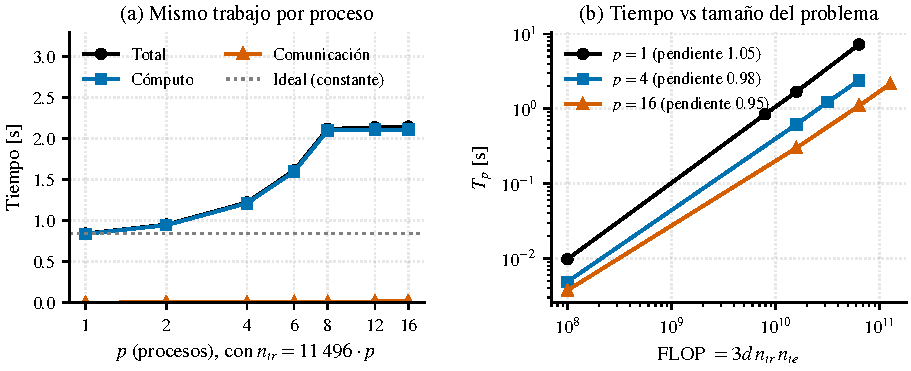
\includegraphics[width=\textwidth]{escalabilidad}
\caption{(a) Serie con el mismo trabajo por proceso ($\ntr=11\,496\cdot p$, $\nte=3600$): si escalara perfecto, el tiempo sería constante (línea punteada). (b) Tiempo frente al trabajo con $p$ fijo, en escala log-log: una pendiente de 1 significa que el tiempo es proporcional al trabajo.}
\label{fig:escala}
\end{figure}

\textbf{Mismo trabajo por proceso} (Fig.~\ref{fig:escala}a; escalabilidad débil o de Gustafson, U2.1). Si $\ntr$ crece al mismo ritmo que $p$, el tiempo ideal es constante. Lo medido sube de 0.84\,s a 2.15\,s, así que la eficiencia $T_1/T_p$ baja a 0.39 con $p=16$. La subida se debe al cómputo (de 0.84 a 2.11\,s). La comunicación crece de 2 a 19\,ms, menos del 1\,\% del total.

\textbf{Tiempo proporcional al trabajo} (Fig.~\ref{fig:escala}b). Con $p$ fijo, las pendientes en escala log-log son 1.05, 0.98 y 0.95 para $p=1$, 4 y 16. Es decir, $T_p$ crece linealmente con $\ntr\nte d$, como predice la complejidad $O(\ntr\nte d/p)$.

\textbf{Isoeficiencia} (U6.2). La función de overhead es $T_0=pT_p-W$. Con la Ec.~(\ref{eq:tp}) y $W=A$:
\[
T_0\approx B\,p^2+C\,p\log_2p+D\,p,\qquad E=\frac{1}{1+T_0/W}.
\]
Domina el término $B\,p^2$, que viene del Gather y de la fusión en $P_0$. Para mantener $E$ constante, el trabajo $W$ debe crecer como $p^2$. En la práctica, el overhead del algoritmo es pequeño: la comunicación nunca supera el 2.5\,\% del tiempo en los conjuntos grandes. Lo que limita la eficiencia medida es el cómputo compartido del nodo (Sec.~\ref{sec:tiempos}), que esta fórmula no incluye.

\subsection{Exactitud del modelo (accuracy)}\label{sec:acc}
Para un mismo conjunto de datos, la exactitud es \textbf{idéntica para todo $p$}, porque las predicciones son las mismas (Sec.~\ref{sec:pseudo}). La Tabla~\ref{tab:acc} muestra que al aumentar los datos la exactitud se mantiene.

\begin{table}[htbp]
\centering\small
\caption{Exactitud (igual para todo $p$).}\label{tab:acc}
\begin{tabular}{@{}lrrr@{}}\toprule
Conjunto & $\ntr$ & $\nte$ & Exactitud\\\midrule
load\_digits (original) & 1437 & 360 & 0.9833\\
Aumentado & 11\,496 & 3600 & 0.9814\\
Mediano & 22\,992 & 3600 & 0.9828\\
Grande & 91\,968 & 3600 & 0.9811\\
Aumentado (máximo) & 183\,936 & 3600 & 0.9817\\\bottomrule
\end{tabular}
\end{table}

\subsection{Comparación con la distribución de la entrega parcial}\label{sec:variantes}
beta3 también permite la distribución de la entrega parcial (Bcast de $X_{tr}$ y Scatter de $X_{te}$). Las comparamos con el conjunto Grande y $p=16$:

\begin{table}[htbp]
\centering\small
\caption{Distribución del DAG frente a la de la entrega parcial (conjunto Grande, $p=16$).}\label{tab:var}
\begin{tabular}{@{}lrrr@{}}\toprule
Distribución & Lo que se difunde (Bcast) & $\tsub{comm}$ [ms] & $T_p$ [s]\\\midrule
DAG del enunciado (final) & $X_{te}$: 1.8\,MB & 11.5 & 1.091\\
Entrega parcial & $X_{tr}$: 47.8\,MB & 53.6 & 1.184\\\bottomrule
\end{tabular}
\end{table}

Con el DAG la comunicación es 4.7 veces menor, porque se difunde $X_{te}$ (pequeño) y no $X_{tr}$ (grande). Por eso, cuando $\ntr\gg\nte$, conviene repartir $X_{tr}$ como indica el DAG.

\subsection{Mejoras propuestas}\label{sec:mejoras}
\begin{enumerate}
\item \textbf{Usar más nodos con menos procesos por nodo.} Lo medido es que el cómputo por proceso se hace más lento al llenar el nodo, y la causa probable es la memoria compartida (U1.1, U4.5). Repartir los procesos en varios nodos le daría a cada uno más ancho de banda de memoria, y además serviría para comprobar esa causa.
\item \textbf{Reducción en árbol de los candidatos (U6.1).} Elegir los $k$ menores es una operación asociativa, como el mínimo. Una reducción en árbol cuesta $O(\log p)$ en vez del $O(p)$ del Gather más la fusión en $P_0$, y quitaría el término $B\,p$ que fija $p^*$.
\item \textbf{Comunicación no bloqueante (U3.3).} Con \texttt{Iscatterv}/\texttt{Ibcast} se puede calcular mientras se comunica. La ganancia es pequeña, porque la comunicación es como máximo el 2.5\,\% del tiempo.
\item \textbf{GPU (U6.4).} El cálculo de distancias es un producto de matrices, ideal para GPU.
\end{enumerate}

% =====================================================================
\section{Conclusiones}
\begin{itemize}
\item El KNN paralelo según el DAG del enunciado es correcto: da exactamente las mismas predicciones que el código original para cualquier $p$ (129/129 comprobaciones).
\item Con 16 procesos y el conjunto Grande alcanza $S=6.61$, $E=0.41$ y 58.3\,GFLOP/s.
\item La complejidad teórica se cumple en dos cosas: el tiempo crece linealmente con el trabajo (pendientes de 0.95 a 1.05) y la comunicación sigue las fórmulas de U6.1 y es muy pequeña.
\item La cantidad óptima de procesos es $p^*\approx\sqrt{A/B}$: unos 8 para \texttt{load\_digits}, lo que coincide con lo medido, y los 16 núcleos para los conjuntos grandes.
\item La eficiencia no llega al ideal por el cómputo y no por la comunicación MPI: con todos los procesos en un mismo nodo, cada uno calcula más lento. La causa probable es la memoria compartida, aunque sin contadores de hardware no podemos confirmarlo.
\end{itemize}

% =====================================================================
\section{Bibliografía y uso de fuentes externas}
\subsection{Material del curso}
Todas las fórmulas del informe salen de las diapositivas del curso \cite{fiestas}:
\begin{itemize}\setlength{\itemsep}{0pt}
\item \textbf{U1.1:} \emph{memory wall}, el acceso a memoria como cuello de botella (Sec.~\ref{sec:tiempos}).
\item \textbf{U1.2:} metodología de Foster y clasificación de Flynn (Sec.~2.1).
\item \textbf{U1.3:} DAG secuencial-paralelo, trabajo $W$ y span $T_\infty$ (Ec.~\ref{eq:work}).
\item \textbf{U2.1:} speedup, eficiencia, escalabilidad fuerte y débil, y rango de GFLOP/s por núcleo.
\item \textbf{U2.2:} PRAM CREW, \texttt{pardo} y teorema de Brent (Alg.~\ref{alg:pram}, Ec.~\ref{eq:brent}).
\item \textbf{U2.4:} particionamiento de datos con tareas separables.
\item \textbf{U3.1--U3.3:} colectivas MPI y comunicación no bloqueante.
\item \textbf{U4.5:} límites por ancho de banda de memoria e hyper-threading (SMT).
\item \textbf{U6.1:} costos de Bcast, Scatter y Gather (Ec.~\ref{eq:comm}), reducción en árbol y el cálculo de un óptimo derivando el tiempo.
\item \textbf{U6.2:} conteo de FLOP, función de overhead $T_0$ e isoeficiencia.
\item \textbf{U6.3:} distancias como producto de matrices. \textbf{U6.4:} GPU.
\end{itemize}

\subsection{Otras fuentes}
\begin{itemize}\setlength{\itemsep}{1pt}
\item \textbf{Enunciado \cite{enunciado}:} código de partida, DAG y preguntas a)--e).
\item \textbf{Fix y Hodges \cite{fix1951}, Cover y Hart \cite{cover1967}:} definición de KNN.
\item \textbf{scikit-learn \cite{sklearn}:} conjunto \texttt{load\_digits} y \texttt{train\_test\_split}.
\item \textbf{NumPy \cite{numpy} y mpi4py \cite{mpi4py}:} producto de matrices, \texttt{argpartition} y colectivas MPI en Python.
\item \textbf{Documentación de Khipu \cite{khipu}:} uso de Slurm y de los módulos del clúster.
\end{itemize}

\subsection{Uso de herramientas de asistencia y modelos de lenguaje}
Declaramos el uso del modelo de lenguaje Claude \cite{claude} (mediante Claude Code) como apoyo (Tabla~\ref{tab:ia}).

\begin{table}[H]
\centering\small
\caption{Declaración de uso de IA.}\label{tab:ia}
\begin{tabularx}{\linewidth}{@{}>{\raggedright\arraybackslash}p{3.1cm}>{\raggedright\arraybackslash}X>{\raggedright\arraybackslash}X@{}}\toprule
\textbf{Uso} & \textbf{Aporte} & \textbf{Control de los autores}\\\midrule
Revisión analítica & Sugerencias sobre el modelo $T_p=A/p+Bp+C\log_2p+D$ y el cálculo de $p^*$. & Derivaciones verificadas a mano con las fórmulas de U2.2, U6.1 y U6.2.\\\addlinespace
Código de análisis y gráficas & Scripts que leen los CSV de Khipu y generan tablas y figuras. & Las cifras se comprobaron con los CSV originales.\\\addlinespace
Redacción y \LaTeX & Estructura y simplificación del informe, pseudocódigos y DAG en TikZ. & Contenido revisado y compilado por los autores.\\\bottomrule
\end{tabularx}
\end{table}

\textbf{Impacto.} La herramienta agilizó la revisión, el análisis y la redacción. Las mediciones provienen de los jobs de Khipu, y las decisiones de diseño y las conclusiones son de los autores.

\begin{thebibliography}{99}\small
\bibitem{fiestas} J.~Fiestas, diapositivas de las unidades U1--U6, CS4052 Computación Paralela y Distribuida, UTEC, 2026.
\bibitem{enunciado} J.~Fiestas, ``Proyecto -- Laboratorio CS4052 2026-II, Sec.~5 (KNN),'' UTEC, 2026.
\bibitem{fix1951} E.~Fix and J.~L.~Hodges, ``Discriminatory analysis: Nonparametric discrimination, consistency properties,'' USAF School of Aviation Medicine, Tech. Rep.~4, 1951.
\bibitem{cover1967} T.~M.~Cover and P.~E.~Hart, ``Nearest neighbor pattern classification,'' \emph{IEEE Trans. Inf. Theory}, vol.~13, no.~1, pp.~21--27, 1967.
\bibitem{sklearn} F.~Pedregosa \emph{et al.}, ``Scikit-learn: Machine learning in Python,'' \emph{JMLR}, vol.~12, pp.~2825--2830, 2011.
\bibitem{numpy} C.~R.~Harris \emph{et al.}, ``Array programming with NumPy,'' \emph{Nature}, vol.~585, pp.~357--362, 2020.
\bibitem{mpi4py} L.~Dalcín, ``MPI for Python (mpi4py),'' \url{https://mpi4py.readthedocs.io/en/stable/}.
\bibitem{khipu} UTEC, ``Documentación del clúster Khipu,'' \url{https://docs.khipu.utec.edu.pe/}, consultado 20-11-2026.
\bibitem{claude} Anthropic, ``Claude (Claude Code),'' 2026. \url{https://claude.ai}.
\end{thebibliography}

\end{document}
